 \documentclass[12pt]{article}
%% note that some of the references from the answers were changed by hand
%% search for Section and Figure
  \usepackage{wrapfig}
 




\DeclareSymbolFont{extraup}{U}{zavm}{m}{n}
\DeclareMathSymbol{\varheart}{\mathalpha}{extraup}{86}
\DeclareMathSymbol{\vardiamond}{\mathalpha}{extraup}{87}

\newcommand{\Flips}{{\sf Flips}}
 \newcommand{\heads}{H}
 \newcommand{\Heads}{\heads}
 \newcommand{\Tails}{\tails}
 \newcommand{\tails}{T}

\newcommand{\Cards}{{\sf Cards}}
 \newcommand{\clubs}{\clubsuit}
\newcommand{\hand}{\mbox{\textcolor{orange}{{\ding{43}}}}}
\newcommand{\hearts}{\textcolor{red}{\varheartsuit}}
\newcommand{\diamonds}{\textcolor{red}{\vardiamondsuit}}
\newcommand{\spades}{\spade}
\renewcommand{\diamond}{\diamonds}
\newcommand{\heart}{\textcolor{red}{\varheartsuit}}
\newcommand{\club}{\clubsuit}
\renewcommand{\diamond}{\diamondsuit}
\newcommand{\spade}{\spadesuit}
\newcommand{\T}{\true}
\newcommand{\F}{\false}
\newcommand{\provesH}{\vdash_{\!\!  \lower3pt\hbox{$\scriptstyle \sf H$}}}

\newcommand{\allsubscript}[1]{#1_{\forall}}
\newcommand{\somesubscript}[1]{#1_{\exists}}
\newcommand{\pall}{\allsubscript{p}}
\newcommand{\psome}{\somesubscript{p}}
\newcommand{\vall}{\allsubscript{v}}
\newcommand{\vsome}{\somesubscript{v}}
\newcommand{\qall}{\allsubscript{q}}
\newcommand{\qsome}{\somesubscript{q}}
\newcommand{\uall}{\allsubscript{u}}
\newcommand{\usome}{\somesubscript{u}}




\newcommand{\RCA}{\mathcal{RCA}}
\newcommand{\RAA}{\mbox{\sc RAA}}
\newcommand{\Lex}{\mbox{\em Lex}}
\newcommand{\N}{\protect{\mbox{N}}}
\newcommand{\vbarsem}[1]{[\![ #1 ]\!]_v}
\newcommand{\wbarsem}[1]{[\![ #1 ]\!]_w}



%\newcommand{\NP}{\protect{\mbox{NP}}}

\newcommand{\binaryterms}[2]{\mbox{\sf All $#1$ are $#2$}}
\newcommand{\cat}{\mbox{\sf cat}}
\newcommand{\dog}{\mbox{\sf dog}}
\newcommand{\see}{\mbox{\sf see}}
\newcommand{\student}{\mbox{\sf student}}
\newcommand{\hear}{\mbox{\sf hear}}
\newcommand{\Amina}{\mbox{\sf Amina}}
\newcommand{\Bao}{\mbox{\sf Bao}}
\newcommand{\skunk}{\mbox{\sf skunk}}
\newcommand{\mammal}{\mbox{\sf mammal}}
\newcommand{\fear}{\mbox{\sf fear}}
\newcommand{\respect}{\mbox{\sf respect}}

\newcommand{\sfbigger}{\mbox{\sf bigger}}

\newcommand{\X}{\mathcal{X}}
\newcommand{\VP}{{\sc VP}}
\newcommand{\propp}{\mbox{\sf p}}
\newcommand{\propq}{\mbox{\sf q}}
\newcommand{\propr}{\mbox{\sf r}}
\newcommand{\SL}{\mbox{\sf SL}}
\newcommand{\eps}{\varepsilon}
\newcommand{\bluedot}{\mbox{\textcolor{blue}{$\bullet$}}}
\newcommand{\reddot}{\mbox{\textcolor{red}{$\bullet$}}}
\newcommand{\yellowdot}{\mbox{\textcolor{yellow}{$\bullet$}}}
\newcommand{\greendot}{\mbox{\textcolor{green}{$\bullet$}}}
\newcommand{\sfevery}{\mbox{\sf every}}
\newcommand{\sfsome}{\mbox{\sf some}}
\newcommand{\sfno}{\mbox{\sf no}}
\newcommand{\sffascinate}{\mbox{\sf fascinate}}
\newcommand{\sfcaptivate}{\mbox{\sf captivate}}
\newcommand{\sfinterest}{\mbox{\sf interest}}
\newcommand{\sfbaby}{\mbox{\sf baby}}
\newcommand{\sfchild}{\mbox{\sf child}}
\newcommand{\sfsee}{\mbox{\sf see}}
\newcommand{\sfperson}{\mbox{\sf person}}
\newcommand{\sfatleasttwo}{\mbox{\sf at least two}}
\newcommand{\posetP}{\mathbb{P}}
\newcommand{\posetM}{\mathbb{M}}
\newcommand{\posetQ}{\mathbb{Q}}
\newcommand{\posetR}{\mathbb{R}}
\newcommand{\posetX}{\mathbb{X}}
\newcommand{\posetBool}{\mathbb{2}}
\newcommand{\Cat}{\cal{C}}
\newcommand{\lookleft}{\backslash}
\newcommand{\lookright}{\slash}
\newcommand{\done}{\infer{\mbox{\sf Some  $p$  are  $n$}}
{\mbox{\sf Some  $n$  are  $p$ }}}

\newcommand{\dthree}{\infer{\done}{{\mbox{\sf All $n$ are $p$}} & 
\mbox{\sf Some $n$ are $n$}  }}
\newcommand{\Rdag}{\cR^\dag}
\newcommand{\cRdag}{\cR^\dag}
\newcommand{\Sdag}{\cS^\dag}
\newcommand{\cSdag}{\cS^\dag}
\newcommand{\cSdagbc}{\cS^\dag_{bc}}
\newcommand{\Sdagbc}{\cS^\dag_{bc}}
\newcommand{\Sdagleq}{\cS^\dag(\mbox{card})}
\newcommand{\Sleq}{\cS(\mbox{card})}

\newcommand{\Allwhichlong}[3]
{\mbox{\sf All $#1$ which are $#2$ are $#3$}}

\newcommand{\Allwhich}[3]
{(#1,#2,#3)}
%\newcommand{\qed}{\relax}
\renewcommand{\theequation}{\arabic{equation}}
\renewcommand{\thefigure}{\arabic{figure}}
\renewcommand{\AA}{{\cal A}}

\newcommand{\abar}{\overline{a}}
\newcommand{\bbar}{\overline{b}}
\newcommand{\cbar}{\overline{c}}
\newcommand{\dbar}{\overline{d}}
\newcommand{\ebar}{\overline{e}}
\newcommand{\gbar}{\overline{g}}
\renewcommand{\hbar}{\overline{h}}
\newcommand{\tbar}{\overline{t}}
\newcommand{\ubar}{\overline{u}}
\newcommand{\aprimebar}{\overline{a}'}
\newcommand{\bprimebar}{\overline{b}'}
\renewcommand{\phi}{\pphi}
 \newcommand{\abovearrow}[1]{\rightarrow\hspace{-.12in}\raisebox{1.0ex}
{$\scriptstyle{#1}$}\hspace{.1in}}

\newcommand{\arrowa}{\,\lower1pt\hbox{$\abovearrow{\!\! a}$}\!\!}
\newcommand{\arrowc}{\,\lower1pt\hbox{$\abovearrow{\!\!c}$}}
\newcommand{\arrowd}{\,\lower1pt\hbox{$\abovearrow{\!\!d}$}}
\newcommand{\arrowdd}{\,\lower1pt\hbox{$\abovearrow{\!\!\!\!dd}$}}
\newcommand{\arrowAB}{\lower1pt\hbox{$\abovearrowlong{\!\!\!\!{AB}}$}}
\newcommand{\arrowe}{\,\lower1pt\hbox{$\abovearrow{\!\!e}$}}


\newcommand{\arrowGamma}{\rightarrow\hspace{-.18in}\raisebox{-1.0ex}
{$\scriptstyle\Gamma$}\hspace{.1in}}
\newcommand{\arrowGammastar}{\rightarrow\hspace{-.18in}\raisebox{-1.0ex}
{$\scriptstyle\Gamma$}
\hspace{-.06in}\raisebox{.8ex}{$\scriptstyle *$}
\hspace{.1in}}
\newcommand{\arrowstar}{\rightarrow\hspace{-.1in}  %was -.18
%\raisebox{-1.0ex}
%{$\scriptstyle\Gamma$}
\hspace{-.06in}\raisebox{.8ex}{$\scriptstyle *$}
\hspace{.1in}}
\newcommand{\arrowGammadoublestar}{\rightarrow\hspace{-.18in}\raisebox{-1.0ex}
{$\scriptstyle\Gamma$}
\hspace{-.09in}\raisebox{.8ex}{$\scriptstyle **$}
\hspace{.1in}}

%\newcommand{\arrowstar}{\rightarrowstar}
\newcommand{\rightarrowstar}{\abovearrow{{*}}}
\newcommand{\arrowpi}{\abovearrow{\pi}}
\newcommand{\Type}{\Types}
\newcommand{\Types}{\mathcal{T}}
\newcommand{\toplussmall}{\longabovearrow{\scriptscriptstyle{\hspace{.07in}+}}}
\newcommand{\tominussmall}{\longabovearrow{\scriptscriptstyle{\hspace{.07in}-}}}
\newcommand{\toplus}{\longabovearrow{+}}
\newcommand{\tominus}{\longabovearrow{-}}
\newcommand{\tostar}{\longabovearrow{*}}
\newcommand{\longabovearrow}[1]{\longrightarrow\hspace{-.2in}\raisebox{1.0ex}
{$\scriptstyle{#1}$}\hspace{.1in}}
\newcommand{\pol}{\mbox{pol}}
\renewcommand{\o}{\cdot}
\newcommand{\arrowx}{\abovearrow{x}}
\newcommand{\arrowy}{\abovearrow{y}}
\newcommand{\arrowz}{\abovearrow{z}}

\newcommand{\addthm}[1]{\relax}
\newcommand{\AtProg}{{\sf AtProg}}
\newcommand{\AtProp}{{\sf AtSen}}
\newcommand{\AtSen}{\AtProp}
\newcommand{\PL}{\sf Sen}
\newcommand{\Sen}{\sf Sen}
\newcommand{\afa}{\mbox{\it AFA}}
\newcommand{\AFA}{\mbox{\it AFA}}
\newcommand{\Agents}{{\sf Ag}}
\newcommand{\al}{\alpha}
\newcommand{\alhf}{\check{\hf}}

\newcommand{\alg}{{\cal A}}
\newcommand{\andd}{\wedge}
\newcommand{\apg}{{\cal S}}
\newcommand{\apgzero}{{\cal S}_0}
\newcommand{\app}[2]{\mbox{$#1^{#2}$}}
%\newcommand{\ar}{\rightarrow}
\newcommand{\arity}{{\it arity}}
\newcommand{\arityfun}{{\it arity_{\it fun}}}
\newcommand{\arityrel}{{\it arity_{\it rel}}}
\newcommand{\atoms}{\Atoms}
\newcommand{\Automaton}{{\cal A}}

\newcommand{\B}{{\catfont B}}
\renewcommand{\H}{{\catfont H}}
\newcommand{\E}{{\catfont E}}

\newcommand{\BB}{{\cal B}}
\newcommand{\DD}{{\cal D}}

\newcommand{\bb}{{\cal P}}
 \newcommand{\belowarrow}[1]{\longrightarrow\hspace{-.24in}\raisebox{-1.4ex}
{$\scriptstyle{#1}$}\hspace{.1in}}
\newcommand{\bfm}[1]{\mbox{\boldmath$#1$\unboldmath}}
%%%% \newcommand{\bfm}[1]{\mbox{\boldmath #1}}
%%% the first \bfm command is better
\newcommand{\bisim}[2]{\mbox{$#1 \approx #2$}}
\newcommand{\Bool}{{\sf Bool}}
\newcommand{\bool}{{\sf Bool}}
\newcommand{\bt}{\bullet}
%\renewcommand{\bullet}{\star}

\newcommand{\catfont}[1]{{\sf #1}}
%\newcommand{\card}[1]{{\rm card}(#1)}
\newcommand{\card}[1]{\cardinal{#1}}
\newcommand{\cardinal}[1]{|#1|}
\renewcommand{\check}[1]{\stackrel{\scriptscriptstyle\vee}{#1}}
\newcommand{\CH}{{\em CH}}
\newcommand{\children}{\mbox{\it children}}
\newcommand{\CC}{{\cal C}}
\newcommand{\C}{{\catfont C}}
\newcommand{\cc}{{\cal C}}
\newcommand{\cl}[1]{\overline{#1}}
\newcommand{\cczero}{\cc_0}
\newcommand{\cod}{{\it cod \/}\ }
\newcommand{\cont}{continuous}
\newcommand{\concat}[2]{#1 ^{\frown} #2}
\newcommand{\coppy}{{\it copy}}
\newcommand{\corecfn}{\varphi}
\newcommand{\corecfnalt}{\psi}

%\newcommand{\csq}[8]
%{
%\begin{picture}(140,140)(-143,0)
%\setlength{\unitlength}{1 pt} 
%\put(0,90){\vector(0,-1){80}}
%\put(10,0){\vector(1,0){75}}
%\put(100,90){\vector(0,-1){80}}
%\put(10,100){\vector(1,0){75}}
%\put(0,100){\makebox(0,0)[c]{$#1$}}  %upper left
%\put(100,100){\makebox(0,0)[c]{$#2$}} %upper right
%\put(0,0){\makebox(0,0)[c]{$#3$}}  %lower left
%\put(100,0){\makebox(0,0)[c]{$#4$}} %lower right
%\put(50,110){\makebox(0,0)[c]{$#5$}} %top side
%\put(-10,50){\makebox(0,0)[r]{$#6$}}  %left side
%\put(50,-10){\makebox(0,0)[c]{$#7$}} %bottom side
%\put(110,50){\makebox(0,0)[l]{$#8$}} %right side
%\end{picture}


\newcommand{\csq}[8]
{\begin{diagram}[tight,size=4em]
 #1             &   \rTo^{#5}    &  #2 \\
\dTo^{#6\ }   &                   &   \dTo_{\ #8} \\
#3           &     \rTo_{#7}  &  #4 \\
\end{diagram}
}

\newcommand{\csqdashtop}[8]
{
\begin{picture}(140,140)(-143,0)
\setlength{\unitlength}{1 pt} 
\put(0,90){\vector(0,-1){80}}
%%\put(10,0){\vector(1,0){75}}
\put(9,100){\line(1,0){11}}
\put(32,100){\line(1,0){11}}
\put(54,100){\line(1,0){11}}
\put(76,100){\vector(1,0){11}}
\put(100,90){\vector(0,-1){80}}
\put(10,0){\vector(1,0){75}}
\put(0,100){\makebox(0,0)[c]{$#1$}}  %upper left
\put(100,100){\makebox(0,0)[c]{$#2$}} %upper right
\put(0,0){\makebox(0,0)[c]{$#3$}}  %lower left
\put(100,0){\makebox(0,0)[c]{$#4$}} %lower right
\put(50,110){\makebox(0,0)[c]{$#5$}} %top side
\put(-10,50){\makebox(0,0)[r]{$#6$}}  %left side
\put(50,-10){\makebox(0,0)[c]{$#7$}} %bottom side
\put(110,50){\makebox(0,0)[l]{$#8$}} %right side
\end{picture}
}

\newcommand{\Canc}{\Can}
\newcommand{\Can}{\mbox{Canc}}
\newcommand{\Dcat}{{\catfont D}}
\newcommand{\D}{\Delta}
\def\ddate{\ifcase\month\or
 January\or February\or March\or April\or May\or June\or July\or
 August\or September\or October\or November\or December\fi
 \space\nmber\day, \nmber\year}
\newcommand{\dd}{\cal D}
  \newcommand{\Def}{{\it Def}}
\newcommand{\degr}[1]{{\rm deg}(#1)}                        

\newcommand{\deno}[3]{\mbox{${\sf Denotes}_{\sf #3}({\sf #1},{\sf #2})$}}
\newcommand{\depth}{\mbox{depth}}
\newcommand{\dmf}{{\it dm\!}_f}
\newcommand{\dirtymark}{\bullet}
\newcommand{\DirtyA}{D_A}
\newcommand{\DirtyB}{D_B}
\newcommand{\DirtyC}{D_C}
\newcommand{\DirtyX}{D_X}
\newcommand{\DirtyY}{D_Y}
\newcommand{\dirty}{\mbox{\tt dirty}}
\newcommand{\vision}{\mbox{\tt vision}}
\newcommand{\father}{\mbox{\tt father}}
\newcommand{\background}{\mbox{\tt background}}
\newcommand{\no}{\mbox{\tt no}}

\newcommand{\dom}{{\it dom  \/}\ }
\newcommand{\down}[1]{\downarrow#1}

\newcommand{\e}{\mbox{$e$}}
\newcommand{\ee}{\EE}
\newcommand{\EE}{{\cal E}}
\newcommand{\EElong}{\tuple{X,A,e}}
\newcommand{\EElongprime}{\tuple{X',A',e'}}
\newcommand{\ep}{\epsilon}
\newcommand{\emptyword}{\epsilon}
\newcommand{\emptystack}{\mbox{\sortfont empty}}
\newcommand{\epsilonA}{\epsilon_{\gothA}}
\newcommand{\epsilonB}{\epsilon_{\gothB}}
\newcommand{\epc}{\epsilon_\cc}
\newcommand{\eqnatoms}[2]{{\it atoms}({#1},{#2})}
\newcommand{\eqnindets}[2]{{\it indets}({#1},{#2})}
\newcommand{\eqnatomsone}[2]{{\it atoms}({#2})}
\newcommand{\eqnindetsone}[2]{{\it indets}({#2})}
\newcommand{\error}{\mbox{\sortfont error}}
\newcommand{\Even}{\mbox{\em Even}}
\newcommand{\fal}{{\sf F}}
\newcommand{\false}{{\sf F}}%%%%% it was{{\bot}}
\newcommand{\falsehood}{f}
\newcommand{\False}{\em False}
\newcommand{\f}{{\cal F}}
%\newcommand{\F}{{\sf F}}
\newcommand{\fbar}{\overline{f}}
\newcommand{\FA}{\mbox{\it FA}}
\newcommand{\FF}{{\cal F}}
\newcommand{\Fraisse}{Fra\"{\i}ss\'{e}}
\newcommand{\fraisse}{\Fraisse}
\newcommand{\Free}{{\it Free\/}}
\newcommand{\freeocc}{\mbox{\em freeocc}}
\newcommand{\ff}{\f}
%\newcommand{\first}[1]{{#1}^0}
\newcommand{\first}{\mbox{$1^{\it st}$}}
 \newcommand{\forces}{\,\mbox{$\mathrel\|\mathrel{\mkern-9mu}-\,$}}
\newcommand{\forcesS}{\mbox{$\mathrel\|^*\mathrel{\mkern-16mu}-\,$}}

\newcommand{\forcessubscript}[1]{\,
           \mbox{$\mathrel\|_{\lower5pt\hbox{$\scriptstyle
                          \bf\sf #1$}}\mathrel{\mkern-19mu}-$}\,}  %%
\newcommand{\forcesJ}{\,
           \mbox{$\mathrel\|_{\lower5pt\hbox{$\scriptstyle
                          \bf\sf J $}}\mathrel{\mkern-17mu}-$}\,} % was 15
\newcommand{\notforcesJ}{\,
           \mbox{$/\mathrel{\mkern-16mu}\mathrel\|_{\lower5pt\hbox{$\scriptstyle
                          \bf\sf J$}}\mathrel{\mkern-17mu}-$}\,}  %% 15
\newcommand{\notforces}{\,\mbox{$\mathrel/\mathrel{\mkern-10mu}
             \mathrel\|\mathrel{\mkern-9mu}-$}\,}  % 5
\newcommand{\notforcessubscript}[1]{\,
           \mbox{$/\mathrel{\mkern-14mu}
                 \mathrel\|_{\lower5pt\hbox{$\scriptstyle
                          \bf\sf #1$}}\mathrel{\mkern-19mu}-$}\,} % 24
\newcommand{\forcesK}{\,
           \mbox{$\mathrel\|_{\lower5pt\hbox{$\scriptstyle
                          \bf\sf K $}}\mathrel{\mkern-20mu}-$}\,} % was 15
\newcommand{\forcesP}{\forcessubscript P}
\newcommand{\notforcesP}{\notforcessubscript P}
\newcommand{\forcesKS}{\mbox{$\mathrel\|^*_{\lower4pt\hbox{$\scriptstyle
                               \kk$}}\mathrel{\mkern-20mu}-\,$}}
\newcommand{\notforcesKS}{\mbox{$\mathrel/\mathrel{\mkern-9mu}
            \mathrel\|^*_{\lower4pt\hbox{$\scriptstyle
                               \kk$}}\mathrel{\mkern-20mu}-\,$}}
\newcommand{\functorf}{\F}
%%%%\renewcommand{\glossary}[1]{#1}
%\newcommand{\G}{\Gamma}
%\newcommand{\Gfinal}{\Gamma^*}
%\newcommand{\Gammalowerstar}{\G_{\!*}}
\newcommand{\G}{{\sf G}}
\newcommand{\Gfinal}{{\overline{\functorf}}}
\newcommand{\Gammalowerstar}{\functorf_{*}}
\newcommand{\GG}{{\cal G}}
\renewcommand{\gg}{\apgzero}
\newcommand{\Godel}{G\"{o}del}
\newcommand{\godel}{\Godel}
\newcommand{\goth}[1]{{\cal #1}}
\newcommand{\gothA}{{\goth{A}}}
\newcommand{\gothB}{{\goth{B}}}
\newcommand{\gothC}{{\goth{C}}}
\newcommand{\gothD}{{\goth{D}}}
\newcommand{\gothE}{{\goth{E}}}
\newcommand{\gothF}{{\goth{F}}}
\newcommand{\gothG}{{\goth{G}}}
\newcommand{\gothH}{{\goth{H}}}
\newcommand{\gothI}{{\goth{I}}}
\newcommand{\gothJ}{{\goth{J}}}
\newcommand{\gothK}{{\goth{K}}}
\newcommand{\gothL}{{\goth{L}}}
\newcommand{\gothM}{{\goth{M}}}
\newcommand{\gothN}{{\goth{N}}}
\newcommand{\gothO}{{\goth{O}}}
\newcommand{\gothP}{{\goth{P}}}
\newcommand{\gothQ}{{\goth{Q}}}
\newcommand{\gothR}{{\goth{R}}}
\newcommand{\gothS}{{\goth{S}}}
\newcommand{\gothT}{{\goth{T}}}
\newcommand{\gothU}{{\goth{U}}}
\newcommand{\gothV}{{\goth{V}}}
\newcommand{\gothW}{{\goth{W}}}
\newcommand{\gothX}{{\goth{X}}}
\newcommand{\gothY}{{\goth{Y}}}
\newcommand{\gothZ}{{\goth{Z}}}
\newcommand{\sfcat}{\mbox{\sf cat}}
\newcommand{\sfdog}{\mbox{\sf dog}}
\newcommand{\sfanimal}{\mbox{\sf animal}}
\newcommand{\sfchase}{\mbox{\sf chase}}
\newcommand{\sfsleeps}{\mbox{\sf sleeps}}
\newcommand{\sfruns}{\mbox{\sf runs}}
\newcommand{\sfany}{\mbox{\sf any}}

\newcommand{\sfatmostone}{\mbox{\sf at most one}}
\newcommand{\sfif}{\mbox{\sf if}}


\newcommand{\preorderB}{\mathbbm{B}}
\newcommand{\preorderP}{\mathbb{P}}
\newcommand{\preorderM}{\mathbbm{M}}
\newcommand{\preorderQ}{\mathbbm{Q}}
\newcommand{\preorderR}{\mathbbm{R}}
\newcommand{\preorderX}{\mathbbm{X}}
\newcommand{\opposite}[1]{-#1}
\newcommand{\preorderBool}{\mathbbm{2}}


\newcommand{\Graph}{{\sf Graph}}
\newcommand{\bPquotient}{\bP\slash{\!\equiv}}
\newcommand{\Literalquotient}{\Literal\slash{\!\equiv}}
\newcommand{\LiteralquotientGamma}{\preorderP_{\Gamma}}
\newcommand{\Literal}{\mbox{\bf Lit}}
\newcommand{\Lit}{\Literal}
\newcommand{\HF}{{\it HF}}
\newcommand{\HH}{{\cal H}}
\newcommand{\HFzero}{\HF^0}
\newcommand{\HFone}{\HF^1}
\newcommand{\HFhalf}{\HF^{1/2}}
\newcommand{\history}{\medskip \subsection*{Historical Remarks}}
\newcommand{\HSnew}{{\it HS}_{\cal N}}
\newcommand{\WFnew}{{\it WF}_{\cal N}}
\newcommand{\states}{\protect{\mbox{\em states}}}
\newcommand{\Barbara}{\mbox{\emph{Barbara}}}
 \newcommand{\Darii}{\mbox{\emph{Darii}}}
 \newcommand{\Antitone}{\mbox{\emph{Antitone}}}
 \newcommand{\Contrad}{\mbox{X}}
 \newcommand{\One}{\mbox{\emph{One}}}
 \newcommand{\Zero}{\mbox{\emph{Zero}}}
 \newcommand{\Someone}{\mbox{\emph{Some}}_1}
 \newcommand{\Sometwo}{\mbox{\emph{Some}}_2}
 \newcommand{\provesindirect}{\vdash_{RAA}}
\newcommand{\provesconfined}{\proves^{\scriptsize \mbox{confined}}}
\newcommand{\implication}[2]{$#2\iif #1$}
\newcommand{\aaa}{\infer {\mbox{\sf All $X'$ are $B'$}}{\infer*{\mbox{\sf All $B$ are $X$}}{}}}
%\newcommand{\bbb}{\infer{\mbox{\sf All $X'$ are $X$}}{\aaa & \mbox{\sf All $B'$ are $X$}}}
\newcommand{\bbb}{\infer{\mbox{\sf All $X'$ are $X$}}{\aaa & \infer*{\mbox{\sf All $B'$ are $X$}}{}}}

\newcommand{\bbbb}{\infer{\mbox{\sf All $Y'$ are  $X$}}{\bbb}}
\newcommand{\ccc}{\infer {\mbox{\sf All $C'$ are $Y'$}}{\infer*{\mbox{\sf All $Y$ are $C$}}{}}}
\newcommand{\ddd}{\infer{\mbox{\sf Some $C'$ are $C'$}}{\mbox{\sf Some $A$ are $C'$}}}
\newcommand{\eee}{\infer{\mbox{\sf Some $C'$ are $Y'$}}{\ccc & \ddd }}
\newcommand{\eeee}{\infer{\mbox{\sf Some $Y'$ are $Y'$}}{\eee }}
\newcommand{\fff}{\infer{\mbox{\sf Some $Y'$ are $X$}}{\bbbb & \eeee }}
%\newcommand{\ggg}{\infer{\mbox{\sf Some $X$ are $Y'$}}{\fff }}
   


\newcommand{\id}{{\it id}}
\newcommand{\Idl}{{\it Idl}}
\newcommand{\idl}{\Idl}
\newcommand{\ii}{i}
\newcommand{\iif}{\rightarrow}
\newcommand{\iiff}{\leftrightarrow}
\newcommand{\ifff}{\leftrightarrow}
\newcommand{\I}{I}
\newcommand{\II}{I\!I}
\newcommand{\imu}{I_{\m}}
\newcommand{\ihm}{I_{H,\m}}
\newcommand{\inu}{I_{\n}}
\newcommand{\ign}{I_{G,\n}}
\newcommand{\inc}{\ \in_{\cc}\ }
\newcommand{\incl}{i}
\newcommand{\inflang}{{\cal L}_{\scriptscriptstyle \infty}}
\newcommand{\integer}{\mbox{\sortfont int}}
\newcommand{\intt}{\mbox{\sortfont int}}
\newcommand{\inv}{{\it invert}}
\newcommand{\istreams}{i_{\scriptstyle str}}
\newcommand{\itrees}{i_{\scriptstyle tr}}
\newcommand{\itf}{{\it iter\!}_f}
\newcommand{\itg}{{\it iter\!}_g}
\newcommand{\ith}{{\it iter\!}_h}
\newcommand{\itH}{{\it iter\!}_H}

%\newcommand{\VP}{{\sc VP}}
\newcommand{\NP}{\mbox{\sc NP}}
\newcommand{\NPs}{\mbox{{\sc  NP}s}}
\newcommand{\Sent}{{\mbox{\sc S}}}
\newcommand{\kkk}{\mbox{\tt k}}
\newcommand{\K}{{K}}
\newcommand{\ka}{\kappa}

\newcommand{\upred}[1]{{#1}^\uparrow}
\newcommand{\downred}[1]{{#1}^\downarrow}
\newcommand{\lb}{{\it lb}}
\newcommand{\leftt}{{\it left\/}\!}
\newcommand{\lts}{{\cal T}}
\newcommand{\LL}{\lang}
\newcommand{\LLL}{\LL_\infty}
\newcommand{\lang}{{\cal L}}
\newcommand{\langMcAGall}{\lang_{MG}(\mbox{\sf all})}
\newcommand{\langMcAGallno}{\lang_{MG}(\mbox{\sf all}, \mbox{\sf no})}
\newcommand{\langMcAGallsomeno}{\lang_{MG}(\mbox{\sf all}, \mbox{\sf some}, \mbox{\sf no})}
\newcommand{\langMcAGallsome}{\lang_{MG}(\mbox{\sf all}, \mbox{\sf some})}
\newcommand{\langMcAGexists}{\lang_{MG}(\mbox{\sf all},\exists)}
\newcommand{\langMcAGnotexists}{\lang_{MG}(\mbox{\sf all},\nott\exists)}
\newcommand{\langallsomeverbs}{\lang(\mbox{\sf all}, \mbox{\sf some}, \mbox{\emph{see}})}
\newcommand{\langallthree}{\lang_{wh}}
\newcommand{\langalllbi}{\lang_{lbi}}
\newcommand{\langall}{\mathcal{A}}
\newcommand{\langsome}{\cS(\mbox{\sf some})}
\newcommand{\langmost}{\lang(\mbox{\sf most})}
\newcommand{\langallexistsgeq}{\lang(\mbox{\sf all},\existsgeq)}
\newcommand{\langallno}{\cS(\mbox{\sf all}, \mbox{\sf no})}
\newcommand{\langallnoexistsgeq}{\lang(\mbox{\sf all}, \mbox{\sf no},\existsgeq)}
\newcommand{\langallsomeno}{\lang(\mbox{\sf all}, \mbox{\sf some}, \mbox{\sf no})}
\newcommand{\langallsomenonames}{\lang(\mbox{\sf all}, \mbox{\sf some}, \mbox{\sf no},
\mbox{names})}
\newcommand{\langallsome}{\cS(\mbox{\sf all}, \mbox{\sf some})}
\newcommand{\langallsomemost}{\lang(\mbox{\sf all}, \mbox{\sf some},\mbox{\sf most})}
\newcommand{\langsomemost}{\lang(\mbox{\sf some},\mbox{\sf most})}
\newcommand{\langsomenames}{\lang(\mbox{\sf some}, \mbox{names})}
\newcommand{\langallsomenames}{\lang(\mbox{\sf all}, \mbox{\sf some}, \mbox{names})}
\newcommand{\langallnonames}{\lang(\mbox{\sf all}, \mbox{\sf no}, \mbox{names})}
\newcommand{\langallsomeexistsgeq}{\lang(\mbox{\sf all}, \mbox{\sf some},\existsgeq)}
\newcommand{\langallsomenoexistsgeq}{\lang(\mbox{\sf all}, \mbox{\sf some},
\mbox{\sf no},\existsgeq)}
\newcommand{\langexists}{\lang(\mbox{\sf all},\exists)}
\newcommand{\langexistsgeq}{\lang(\mbox{\sf all},\existsgeq)}
\newcommand{\langnotexists}{\lang(\mbox{\sf all},\nott\exists)} 
\newcommand{\langallsomecomplement}{\lang(\mbox{\sf all}, \mbox{\sf some},{}')}
\newcommand{\langallsomecomplementbc}{\lang(\mbox{\sf all}, \mbox{\sf some},{}',bc)}

\newcommand{\leqplus}{\leq^{+}}
\newcommand{\lift}[1]{\overline{#1}}
\newcommand{\lm}{{\bf missing point here}}
\newcommand{\lngth}[1]{{\rm lh}(#1)}
\newcommand{\lob}{L\"{o}b}
\newcommand{\Lob}{L\"{o}b}
\newcommand{\logic}{{\sf L}}

\newcommand{\m}{m}
\newcommand{\M}{{\catfont M}}

\newcommand{\Mafa}{M_{{\it afa}}}
\newcommand{\mapf}{{\it map\!}_f}
\newcommand{\Mapf}{{\it Map\!}_f}
\newcommand{\mapg}{{\it map\!}_g}
\newcommand{\mapG}{{\it map\!}_G}

\newcommand{\mm}{{\cal M}}
\newcommand{\MM}{{\cal M}}
\newcommand{\map}[3]{#1\,:#2 \rightarrow #3}
\newcommand{\ntransmap}[3]{#1\,:#2 \rightarrow #3}

\newcommand{\inclusionmap}[3]{#1\,:#2 \hookrightarrow #3}
\newcommand{\modelsG}{\models_G\ }

\newcommand{\modelsall}[1]{\models{\mkern-15mu}\raise5pt\hbox{$\scriptstyle#1$}}

\newcommand{\modelstheory}{\mid\!\models}
                          
\newcommand{\modelsalltheory}[1]{\mid\!\modelsall{#1}}

\newcommand{\md}[1]{{\rm d}_{\poss}(#1)}   
\newcommand{\mody}{\models}
\newcommand{\modn}{\models^-}
\newcommand{\Mon}{{\catfont{Mon}}}
 
\newcommand{\mv}[1]{{\rm mv}(#1)}


   
\newcommand{\n}{n}
\newcommand{\NN}{{\cal N}}
\newcommand{\nec}{\Box}
\newcommand{\necc}{\Box}
\newcommand{\window}{\boxminus}
\newcommand{\nextcardinal}[1]{{\rm hcard}^+(#1)}
\newcommand{\notmpo}{\ \not\mpobasic \ } 
\newcommand{\nott}{\neg}
\newcommand{\noteq}{\neq}
%\newcommand{\notmodels}{\not\models}
%%%% \newcommand{\nullinfon}{\bot}
\newcommand{\nullinfon}{\mbox{$\bot$}}

\newcommand{\num}{\mbox{\sortfont num}}

\renewcommand{\O}{{\catfont O}}
\newcommand{\oo}{{\cal O}}
\newcommand{\occ}{\mbox{\em occ}}
\newcommand{\Odd}{\mbox{\em Odd}}
\newcommand{\On}{\mbox{\it On}}
\newcommand{\Om}{\Omega}
\newcommand{\orr}{\vee}


\newcommand{\p}{n}
\newcommand{\pair}[1]{\langle  #1 \rangle}
\newcommand{\partialmap}[3]{#1\,:#2 \rightharpoonup #3}
\newcommand{\pphi}{\varphi}
\newcommand{\play}[1]{#1^{\leq \infty}}
\newcommand{\plusminus}{\underline{+}\,}
\newcommand{\po}{\sqsubseteq}
\newcommand{\pop}{\mbox{\em pop}}
\newcommand{\pos}{\Diamond}
\newcommand{\poss}{\Diamond}
\newcommand{\pow}{{\cal P}}
\newcommand{\power}{{\cal P}}
\newcommand{\powerfinite}{\wpf}
\newcommand{\pp}{{\cal P}}
\newcommand{\proofend}{{\unskip\nobreak\hfill\ $\dashv$ \par \medbreak}}
\newcommand{\provable}{p}
\newcommand{\proves}{\vdash}
\newcommand{\provese}{\vdash_e}
\newcommand{\provesi}{\vdash_i}
\newcommand{\provesc}{\vdash_c}
\newcommand{\provesie}{\vdash_{ie}}
\newcommand{\provesnew}{\vdash_{\!\!\! new}}
\newcommand{\provesalt}{\vdash_{\!\!\! alt}}
\newcommand{\notproves}{\not\!\vdash}
%%%%% out by csli conflict  \newcommand{\pr}{\proves}
\newcommand{\PS}{{\cal PS}}
\newcommand{\pump}{\pi}
\newcommand{\push}{\mbox{\em push}}

\newcommand{\qq}{{\cal Q}}


%%%%%%%%%%%%%%%%%%%%%%%%%%%%%%%%%%%%%%%%%%%%%%%%%%%%%%%%%%%%%%%%%%
% Put "\Qq", and then curly braces around whatever you want inside
% CORNER-QUOTES (or quine-quotes).  Arguments of \leftsqr and \rightsqr:
% (1) length of lines in ex's
% (2) width of lines in pt's
% (3) raised by in ex's
% (4) overlap in em's

\def\leftsqr#1#2#3#4{{\mathopen{\hbox{\hskip.2em}\raise#3ex\vbox{\hrule
    height.#2pt\hbox{\vrule width.#2pt height #1ex\kern#1ex}}\kern-.#4em}}}
\def\rightsqr#1#2#3#4{{\mathclose{\kern-.#4em\raise#3ex\vbox{\hrule
    height.#2pt\hbox{\kern#1ex \vrule width.#2pt
    height #1ex}}\hbox{\hskip.2em}}}}
\def\leftsquare{\leftsqr{.7}2{1.15}{1}}
\def\rightsquare{\rightsqr{.7}2{1.15}{1}}
\def\Leftsquare{\leftsqr{.7}2{1.45}{2}}
\def\Rightsquare{\rightsqr{.7}2{1.45}{2}}
\def\Qq#1{\ifmmode \leftsquare #1 \rightsquare \else%
		  $\leftsquare$#1$\rightsquare$\fi} 
\def\QQ#1{\ifmmode \Leftsquare #1 \Rightsquare \else%
		  $\Leftsquare$#1$\Rightsquare$\fi}  

%%\newcommand{\qu}[1]{\mbox{$\stackrel{\scriptstyle  \lceil}{}\! #1
%%%  \!\stackrel{\scriptstyle \rceil}{}$}}
\newcommand{\qu}[1]{\Qq{#1}}

%%%%%%%%%%%%%%%%%%%%%%%%%%%% end of stuff on corner quotes %%%%%%%%%

\newcommand{\qualt}[1]{\mbox{`}#1\mbox{'}}
\newcommand{\rem}[1]{\relax}
\newcommand{\quadiff}{\quad \mbox{iff}\quad}
\newcommand{\quadiiff}{\quad \iiff\quad}
\newcommand{\quadeq}{\quad = \quad}
\newcommand{\quadleq}{\quad \leq \quad}
\newcommand{\quadequiv}{\quad \equiv \quad}
\newcommand{\quadsubseteq}{\quad \subseteq \quad}
\newcommand{\Sat}{\mbox{\rm Sat}}
\newcommand{\inl}{{\sf inl}}
\newcommand{\inr}{{\sf inr}}
\newcommand{\rank}{{\rm rank}}
\newcommand{\rb}{{\it rb}}
\newcommand{\rightt}{{\it right\/}\!}
\newcommand{\rk}{\rank}%%%%%%%%%%{\mbox{\sf rank}}
%%%%%%%%  out by csli      \newcommand{\rem}[1]{\relax}
\newcommand{\restr}{\upharpoonright}
%\newcommand{\restr}{\mid}
\newcommand{\rstar}{R^*}
\newcommand{\RR}{{\cal R}}
\newcommand{\sbar}{\overline{s}}
\newcommand{\SSS}{{\cal S}}
\newcommand{\sss}{\mbox{\tt s}}
\newcommand{\sortfont}[1]{\tt #1}
\newcommand{\stack}{\mbox{\sortfont stack}}
\newcommand{\se}{\mbox{$(\Sigma,E)$}}
\newcommand{\sem}{{\cal S}}
%\newcommand{\second}[1]{{#1}^1}
\newcommand{\second}{\mbox{$2^{\it nd}$}}
%\newcommand{\semantics}[1]{[\![ #1 ]\!]}
    \newcommand{\FO}{\mbox{FO}}
\newcommand{\Model}{{\cal M}}
\newcommand{\Nodel}{{\cal N}}
%\newcommand{\MM}{\Model}
\renewcommand{\SS}{{\cal S}}         
\newcommand{\semantics}[1]{[\![\mbox{\em #1\/}]\!]}
\newcommand{\SD}{\mbox{\sf SD}}
\newcommand{\seq}{{\sf seq}}
\newcommand{\set}[1]{\{ #1 \}}
\newcommand{\Set}{{\sf Set}}
\newcommand{\sfe}{{\sf e}}
\newcommand{\sff}{{\sf f}}
\newcommand{\sfg}{{\sf g}}
\newcommand{\sfh}{{\sf h}}
\newcommand{\sfm}{{\sf m}}
\newcommand{\sfn}{{\sf n}}
\newcommand{\sfp}{{\sf p}}
\newcommand{\sfq}{{\sf q}}
\newcommand{\sfr}{{\sf r}}
\newcommand{\sfs}{{\sf s}}
\newcommand{\sft}{{\sf t}}
\newcommand{\sfthis}{{\sf this}}
\newcommand{\sfu}{{\sf u}}
\newcommand{\sfv}{{\sf v}}
\newcommand{\sfw}{{\sf w}}
\newcommand{\sfx}{{\sf x}}
\newcommand{\sfy}{{\sf y}}
\newcommand{\sfz}{{\sf z}}
\newcommand{\sfR}{{\sf R}}
\newcommand{\sfTrue}{{\sf True}}
\newcommand{\sftrue}{{\sf True}}

\newcommand{\sfnew}{{\sf new}}

%%%% the next line has to be removed once the CSLI 
%%%% macros are in place !!!
%%%%
%%%\newcommand{\shcite}{\cite}

\newcommand{\Sfour}{{S4}}
\newcommand{\Sfive}{{S5}}
\newcommand{\si}{\sigma}
\newcommand{\Sigmafun}{\Sigma_{\it fun}}
\newcommand{\Sigmarel}{\Sigma_{\it rel}}
\newcommand{\Sigmabool}{\Sigma_{\it bool}}
\newcommand{\Sigmanat}{\Sigma_{\it nat}}
\newcommand{\skipp}{\bigskip}
\newcommand{\Sigmagraph}{\Sigma_{\it gr}}
\newcommand{\Sigmagr}{\Sigmagraph}
\newcommand{\sideremark}[1]{\noindent{#1}\par} 
%%%%%%%%%%%% To eliminate the side remarks, 
%%%%%%%%%%%% change the above to  \newcommand{\sideremark}[1]{\relax}
\newcommand{\sig}{$\Sigma$}
\newcommand{\solutionset}{\mbox{\it solution-set\/}}
%\newcommand{\so}{sometimes} 
\newcommand{\sub}{{\it sub\/}}
\newcommand{\subsumes}[2]{\mbox{$#1 \sqsubseteq #2$}} 
\newcommand{\supp}[1]{\mbox{${\it support}(#1)$}}
\newcommand{\summ}[2]{\sum_{#1}\ #2}
\newcommand{\sys}{{\bf Sys}}
 \newcommand{\Str}[1]{{#1}^\infty}   

\renewcommand{\t}{{\sf T}} 
\newcommand{\TC}{{\it TC}}
\newcommand{\ttt}{{\cal T}}
\newcommand{\TT}{{\cal T}}
\newcommand{\Theories}{{\it Th}}
\newcommand{\thh}{{\sf th}}
\newcommand{\third}{\mbox{$3^{\it rd}$}}
\newcommand{\Th}{{\cal M}}
\renewcommand{\to}{\rightarrow}
\newcommand{\topp}{\mbox{\em top}}
\newcommand{\topg}{{\rm top}_G}
\newcommand{\toph}{{\rm top}_H}
 \newcommand{\Tr}[1]{{#1}^{\it trees}} 
\newcommand{\tr}[1]{{\rm tr}(#1)}
%%%\newcommand{\tri}[1]{\triangle #1}
\newcommand{\tri}{\triangle}
\newcommand{\trans}[3]{\mbox {$#2 \stackrel{#1}{\longrightarrow} #3$}}
\newcommand{\tru}[2]{\mbox{${\sf True}_{\sf #2}({\sf #1})$}}
\newcommand{\true}{{\sf T}}
\newcommand{\True}{\em True}
\newcommand{\tuple}[1]{\mbox{$\langle #1 \rangle $}} 
\newcommand{\tick}{{\it tick}}
\newcommand{\breakk}{{\it break}}
\newcommand{\clock}{{\it clock}}
\newcommand{\stuckclock}{{\it stuckclock}}

\newcommand{\U}{{\catfont U}}
\newcommand{\uu}{{\cal U}}
\newcommand{\UU}{{\cal U}}
\newcommand{\uuu}{{\cal U}_\infty}
\newcommand{\up}[1]{\uparrow\!#1}
\newcommand{\V}{V}
\newcommand{\Val}{\mbox{\em Val}}
\newcommand{\val}{\Val}
\newcommand{\vv}{{\cal V}}
\newcommand{\VV}{{\cal V}}
\newcommand{\vafa}{V_{{\it afa}}}
\newcommand{\Vafa}{V_{{\it afa}}}
\newcommand{\vbar}{\overline{v}}
\newcommand{\vwf}{V_{{\it wf}}}
\newcommand{\Vwf}{V_{{\it wf}}}
\newcommand{\Vnew}{V_{\cal N}}
\newcommand{\Vmin}{V_{\it min}}
    \newcommand{\pbar}{\overline{p}}
    \newcommand{\zbar}{\overline{z}}
\newcommand{\qbar}{\overline{q}}
\newcommand{\rbar}{\overline{r}}

\newcommand{\wbar}{\overline{w}}
\newcommand{\uulf}{{\cal U}_{\,\sf lf}}
\newcommand{\WF}{{\it WF}}
\newcommand{\Wfd}{{\it Wfd}}
\newcommand{\wpf}{{\cal P}_{\scriptstyle fin}}
\newcommand{\wpbot}{{\wp}^{\bot}}

\newcommand{\xbar}{\overline{x}}
\newcommand{\kbar}{\overline{k}}
\newcommand{\xsubi}{x_i}
\newcommand{\xn}{x_1,\ldots,x_n}
%\newcommand{\X}[1]{{#1}}
\newcommand{\Xrules}{{\mathcal X}}
\newcommand{\XX}{{\cal X}}
\newcommand{\ybar}{\overline{y}}
\newcommand{\YY}{{\cal Y}}
\newcommand{\mbar}{\overline{m}}
\newcommand{\nbar}{\overline{n}}
\newcommand{\ysubj}{y_j}
\newcommand{\ym}{y_1,\ldots,y_m}

\newcommand{\zip}{{\it zip\/}}
\newcommand{\ZFM}{\mbox{{\it ZFC}$^-$}}
\newcommand{\ZFA}{\mbox{\it ZFA}}
\newcommand{\ZFC}{\mbox{\it ZFC}}
\newcommand{\zfc}{\ZFC}
\newcommand{\Zfc}{\ZFC}
\newcommand{\zf}{\mbox{\it ZF}}
\newcommand{\ZF}{\mbox{\it ZF}}
\newcommand{\zfa}{\ZFA}
\newcommand{\zfm}{\ZFM}

\newcommand{\ows}{{\sf ows}}
\newcommand{\sws}{{\sf sws}}
\newcommand{\swstag}[1]{(#1)_{\sws}}
\newcommand{\owstag}[1]{(#1)_{\ows}}






\newcommand{\NLOGSPACE}{\textsc{NLogSpace}}
\newcommand{\NEXPTIME}{\textsc{NExpTime}}
\newcommand{\EXPTIME}{\textsc{ExpTime}}
\newcommand{\PTIME}{\textsc{PTime}}
\newcommand{\NPTIME}{\textsc{NPTime}}

\newcommand{\R}{{\sf R}} %{{\cal X}}
\renewcommand{\S}{{\sf S}} %{{\cal X}}

\hyphenation{Des-cartes}
\hyphenation{well-founded}
\hyphenation{well-order}
\hyphenation{well-orders}
\hyphenation{Etche-mendy}
\hyphenation{Moscho-vakis}
\hyphenation{bi-simu-la-tion}
\hyphenation{pleni-tude}


%\newenvironment{examples}{\begin{examp} \rm }{\end{examp}}
%\newenvironment{ex}{\begin{examp} \rm }{\end{examp}}
%\newenvironment{excotd}{\begin{examp} \rm }{\end{examp}}

\newenvironment{definition}{\bigskip\noindent       \pagebreak[1]\bf Definition\ \rm}{\medskip}
\newenvironment{method}{\bigskip\noindent 
        \pagebreak[1]\bf Method of Proof \rm}{\medskip}
%\newenvironment{definitions}{\bigskip\noindent     \pagebreak[1]\bf Definitions\ \rm}{\medskip}
\newenvironment{remark}{\bigskip\noindent        \pagebreak[1]\bf Remark\ \rm}{\medskip}

\newenvironment{claim}{\bigskip\noindent 
        \pagebreak[1]\bf Claim\ \rm}{\medskip}

%\newcounter{excounter}\setcounter{excounter}{0}

\newcounter{examplecounter}\setcounter{examplecounter}{0}




%\newenvironment{example}{\bigskip\noindent              \bf Example\ \rm}{\medskip}
\newenvironment{examples}{\bigskip\noindent 
               \bf Examples\ \rm}{\medskip}


\rem{
\newenvironment{example}{\bigskip\pagebreak[1] \refstepcounter{examplecounter}
          \noindent
{\bf Example\ \theexamplecounter.}\ }{\smallskip}
}

     
\newenvironment{example}{\bigskip\noindent 
        \pagebreak[1]\bf \begin{ex}\ \rm}{\end{ex}\medskip}
        
        
% \newtheorem{thth}{Theorem}[chapter] 
     
%\newenvironment{thm}{\bigskip\noindent 
  %      \pagebreak[1]\bf \begin{thth}\it }{\end{thth}\medskip}
        
        

\newtheorem{theorem}{Theorem}[section] 
\newtheorem{lemma}[theorem]{Lemma}
\newtheorem{proposition}[theorem]{Proposition}
\newtheorem{corollary}[theorem]{Corollary}

%\theoremstyle{definition}
\newtheorem{construction}[theorem]{Construction}
 \newtheorem{ex}[theorem]{Example}

\newtheorem{notation}[theorem]{Notation}
\newtheorem{proj}{Project}
%\newtheorem{exer}{Exercise} 
\newtheorem{fact}{Fact} 
\newtheorem{examp}{Example}
        
 \newcounter{excounter}

%\renewcommand\theexcounter{\thechapter.\arabic{equation}}
\setcounter{excounter}{0}
%\newtheorem{exer}{Exercise}[section]
\newenvironment{exer}{\bigskip\pagebreak[1]  
 \refstepcounter{excounter}
          \noindent  
{\bf Exercise \theexcounter.}\ }{\smallskip}       
 
\rem{        
\newenvironment{exer}{\bigskip\pagebreak[1] \refstepcounter{excounter}
          \noindent
{\bf Exercise\ \theexcounter.}\ }{\smallskip}
}
\newcommand{\jone}{\infer[\AItag^1]{\forall(d,a)(j)}{\jtwo}}
\newcommand{\jtwo}{\infer[\transtag]{a(j,x)}{a(j,k) & \jthree}}
\newcommand{\jthree}{\infer[\AEtag]{a(k,x)}{[d(x)]^1 & \forall(d,a)(k)}}




\newenvironment{answer}{
\bigskip\pagebreak[1] 
          \noindent\rm }{\smallskip}

\newenvironment{question}{\bigskip\noindent 
        \pagebreak[1]\bf Question\ \rm}{\medskip} 



\newcommand{\ans}[1]{\bf #1.\rm\ }

%\newcounter{examplecounter}\setcounter{examplecounter}{0}

%\newenvironment{ex}{\bigskip\pagebreak[1] \refstepcounter{examplecounter}
%          \noindent
%{\bf Example\  \theexamplecounter.}\ }{\smallskip}

%\newenvironment{excotd}{\bigskip\pagebreak[1] 
      %%%%%%\refstepcounter{examplecounter}
%          \noindent
%{\bf Example\ \theexamplecounter, continued.}\ }{\smallskip}

%\newenvironment{exnonumber}{\bigskip\pagebreak[1]
%\noindent
%{\bf Example\ }\ }{\smallskip}

%\renewcommand{\labelenumi}{(\roman{enumi})}


%\newenvironment{proof}{\noindent \bf Proof \ \rm}{ {\unskip\nobreak\hfill\ $\dashv$ \par \medbreak}}


%%%%% special commands to get a name index only %%%

\newcommand{\Rstar}{\mbox{\sf{RC}}}
\newcommand{\Rstartr}{\Rstar(\sf{tr})}
\newcommand{\Rstartrirr}{\mbox{\sf{R}}{}^*{{\sf(tr,irr)}}}
\newcommand{\Rstartrconv}{\mbox{\sf{RC}}{{\sf(tr,conv)}}}
\newcommand{\Rstartrirropp}{\mbox{\sf{RC}}{{\sf(tr,irr,conv)}}}
\newcommand{\Rstartrirrfin}{\mbox{\sf{RC}}{{\sf(tr,irr,fin)}}}
\newcommand{\Rtr}{\mbox{\sf{R}}{{\sf(tr)}}}
\newcommand{\Rtrconv}{\mbox{\sf{R}}{{\sf(tr,conv)}}}
\newcommand{\Gammamost}{\Gamma_{\scriptstyle most}}
\newcommand{\Gammanew}{\Gamma_{\scriptstyle  new}}
\newcommand{\Gammaold}{\Gamma_{\scriptstyle  old}}
\newcommand{\Gammanames}{\Gamma_{\scriptstyle  names}}
\newcommand{\Gammaall}{\Gamma_{\scriptstyle all}}
\newcommand{\Gammaallno}{\Gamma_{\scriptstyle all,no}}
\newcommand{\Gammaallsome}{\Gamma_{\scriptstyle all,some}}
\newcommand{\Gammanotall}{\Gamma_{\nott\scriptstyle all}}
\newcommand{\Gammasome}{\Gamma_{\scriptstyle some}}
\newcommand{\Gammano}{\Gamma_{\scriptstyle no}}
\newcommand{\Gammaat}{\Gamma_{\scriptstyle at}}
\newcommand{\Gammaatneg}{\Gamma_{\scriptstyle \plusminus at}}
\newcommand{\Gammabar}{\overline{\Gamma}}
\newcommand{\existsgeq}{\exists^{\geq}}
\newcommand{\existsmore}{\exists^{>}}
\newcommand{\more}{\exists^{>}}
\newcommand{\leqc}{\leq_c}
\newcommand{\equivc}{\equiv_c}

\newcommand{\leqmore}{\leq_{more}}
\newcommand{\leqmorestrict}{<_{more}}
\newcommand{\nameindex}[1]{\index{#1}}
\newcommand{\uar}{\uparrow}

\newcommand{\proofsystem}[1]{\mbox{\sf #1}}
\newcommand{\logicsystem}[1]{\proofsystem{#1}}
  
\newcommand{\bbP}{{\mathbb{P}}}
\newcommand{\bN}{{\mathbf{N}}} 
\newcommand{\bP}{{\mathbf{P}}}  % Mathbold P (set of unary predicates)
\newcommand{\bQ}{{\mathbf{Q}}}  % Mathbold P (set of unary predicates)
\newcommand{\bA}{{\mathbf{A}}}  % Mathbold P (set of unary predicates)
\newcommand{\bR}{{\mathbf{R}}}  % Mathbold R (set of binary predicates)
\newcommand{\bK}{{\mathbf{K}}}  % Mathbold R (set of constants)
\newcommand{\bC}{{\mathbf{C}}}  % Mathbold C (set of c-terms
\newcommand{\cF}{{\mathcal{F}}}  % Caligraphic F (fragments of FOL)
\newcommand{\cL}{{\mathcal{L}}}  % Caligraphic L (fragments of FOL)
\newcommand{\cS}{\protect{\mathcal{S}}}  % Caligraphic S (syllogistic)
\newcommand{\cR}{{\mathcal{R}}}  % Caligraphic R (rel syllogistic)
\newcommand{\cRstar}{{\mathcal{RC}}}
\newcommand{\RC}{\cRstar}
\newcommand{\cRstardagger}{\cRstar^{\dagger}}
\newcommand{\fA}{\fM} %%%{\mathfrak{M}}}  % Fraktur A (structure)
\newcommand{\fB}{{\mathfrak{B}}}  % Fraktur B (structure)
\newcommand{\fC}{{\mathfrak{C}}}  % Fraktur C (structure)
\newcommand{\fM}{{\cal{M}}}%{{\mathfrak{M}}}  % Fraktur C (structure)
\newcommand{\genProves}{\mid \hspace{-0.06cm}\sim}
 \renewcommand{\k}{j}
 \newcommand{\kprime}{k}   
     \newcommand{\kdoubleprime}{l}   
\newcommand{\betaone}[3]{\forall(#1,\forall(#2,#3))}
\newcommand{\betatwo}[3]{\forall(#1,\exists(#2,#3))}
\newcommand{\betathree}[3]{\exists(#1,\forall(#2,#3))}
\newcommand{\betafour}[3]{\exists(#1,\exists(#2,#3))}
 
\newcommand{\phibar}{\overline{\phi}}
\newcommand{\psibar}{\overline{\psi}}

 \newcommand{\Sub}{\mbox{\emph{Sub}}}  

\newcommand{\obar}{\overline{o}}

\newlength{\mathfrwidth}
  \setlength{\mathfrwidth}{\textwidth}
  \addtolength{\mathfrwidth}{-2\fboxrule}
  \addtolength{\mathfrwidth}{-2\fboxsep}
\newsavebox{\mathfrbox}
\newenvironment{mathframe}
    {\begin{lrbox}{\mathfrbox}\begin{minipage}{\mathfrwidth}\begin{center}\begin{math}\displaystyle}
    {\end{math}\end{center}\end{minipage}\end{lrbox}\noindent\fbox{\usebox{\mathfrbox}}}



\newcommand{\AEtag}{\mbox{\small $\forall E$}}
 \newcommand{\AItag}{\mbox{\small $\forall I$}}
 \newcommand{\EEtag}{\mbox{\small $\exists E$}}
 \newcommand{\EItag}{\mbox{\small $\exists I$}}
  \newcommand{\botItag}{\mbox{\small $\bot I$}}
    \newcommand{\transtag}{\mbox{\small trans}}
        \newcommand{\Xtag}{\protect{\mbox{\small X}}}
 \newcommand{\RAAtag}{\protect{\mbox{\sc RAA}}}

\newcommand{\Modelzero}{\mathcal{P}}
\newcommand{\Modelone}{\mathcal{O}}
\newcommand{\Modeltwo}{\mathcal{N}}
\newcommand{\Modelthree}{\mathcal{M}}

\newcommand{\DangerousBend}
{\begin{wrapfigure}{L}{0.07\textwidth}%% 0.1
\centering
\includegraphics[width=0.04\textwidth]{DangerousBend.png}%% 0.05
\end{wrapfigure} \noindent
}


\newcommand{\GoldStar}
{\begin{wrapfigure}{L}{0.07\textwidth}%% 0.1
\centering
\includegraphics[width=0.04\textwidth]{GoldStar.png}%% 0.05
\end{wrapfigure}
}




\font\manual=manfnt
\def\dbend{{\manual\char127}} % dangerous bend sign

% Danger, Will Robinson!
\newenvironment{danger}{\medbreak\noindent\hangindent=2pc\hangafter=-2%
  \clubpenalty=10000%
    \hbox to0pt{\hskip-\hangindent\dbend\hfill}\ignorespaces}
%  \hbox to0pt{\hskip-\hangindent\dbend\hfill}\small\ignorespaces}%
  {\medbreak\par}

% Danger! Danger!
\newenvironment{ddanger}{\medbreak\noindent\hangindent=3pc\hangafter=-2%
  \clubpenalty=10000%
  \hbox to0pt{\hskip-\hangindent\dbend\kern2pt\dbend\hfill}\small\ignorespaces}%
  {\medbreak\par}


\newenvironment{mydanger}{\medbreak\noindent\hangindent=2pc\hangafter=-2%
  \clubpenalty=10000%
    \hbox to0pt{\hskip-\hangindent\includegraphics[width=0.04\textwidth]{DangerousBend.png}\hfill}\ignorespaces}
%  \hbox to0pt{\hskip-\hangindent\dbend\hfill}\small\ignorespaces}%
  {\medbreak\par}


    \usepackage{proof}
    \usepackage{url}
    \usepackage{fitch}
    \usepackage[all]{xy}  
      \usepackage{enumitem}
%\thispagestyle{empty}
\usepackage{tikz}
\usetikzlibrary{arrows,shapes,snakes,automata,backgrounds,petri,trees}
\usepackage{pifont}
\usepackage{pxfonts} 
\oddsidemargin 0pt
\evensidemargin 0 pt
\topmargin -.3in
\headsep 20pt
\footskip 20pt
\textheight 8.5in
\textwidth 6.25in
%\newcommand{\cal}[1]{\mathcal{#1}}
% Alter some LaTeX defaults for better treatment of figures:
    % See p.105 of "TeX Unbound" for suggested values.
    % See pp. 199-200 of Lamport's "LaTeX" book for details.
    %   General parameters, for ALL pages:
%    \renewcommand{\truefraction}{0.9}	% max fraction of floats at top
%    \renewcommand{\falsetomfraction}{0.8}	% max fraction of floats at bottom
    %   Para meters for TEXT pages (not float pages):
    \setcounter{topnumber}{2}
    \setcounter{bottomnumber}{2}
    \setcounter{totalnumber}{4}     % 2 may work better
    \setcounter{dbltopnumber}{2}    % for 2-column pages
    \renewcommand{\dbltopfraction}{0.9}	% fit big float above 2-col. text
    \renewcommand{\textfraction}{0.07}	% allow minimal text w. figs
    %   Parameters for FLOAT pages (not text pages):
    \renewcommand{\floatpagefraction}{0.7}	% require fuller float pages
	% N.B.: floatpagefraction MUST be less than topfraction !!
    \renewcommand{\dblfloatpagefraction}{0.7}	% require fuller float pages

\newcommand{\sw}{*}
\renewcommand\thesubsection{\arabic{subsection}}

 \begin{document}


\begin{center}
{
\Large  Modal Logic, Winter 2019   \\
   Homework 7
\\
due Tuesday, March 5 \\
} 
\end{center}

\section{Some derivations in $\lang(\sw)$}

\begin{enumerate}
\item $\proves (\nott \phi) \iif (\sw\nott\sw\ \phi)$.
 
\item  $\proves (\sw\nott\sw \phi)\iif (\nott\phi)$.
\item  $\proves \phi \iif  (\nott \sw\nott\sw\ \phi)$.
\end{enumerate}
You can use results from class in your derivations.
But you should say what you're using, and you should be sure that you aren't using more than
what we showed.   That is, if you think you're cutting a corner, please put in the details.

You also can drop the parentheses; usually one would not need parentheses in sentences like (1) above.

\section{Another inductive step in the lemma on $\sw$-$\SD$s}
Here is one of the main 
results on  $\sw$-$\SD$s:

Let $\alpha$ be a $*$-state description (of some order or other).
Let $\occ(\phi) \subseteq\occ(\alpha)$.

 


Then both of the following hold:
\begin{itemize}
\item[1.] Either $\proves \alpha\iif \phi$, or else $\proves \alpha\iif \nott\phi$
\item[2.] Either $\proves \alpha\iif \sw \phi$, or else $\proves \alpha\iif \sw\nott\phi$
\end{itemize}

We prove this by induction on sentences in the language $\lang(\sw)$.
Do the inductive step for $\nott$.   That is, write clearly what you assume and what you prove for that step;
then do the proof.   If some of it is the same as what we saw for propositional logic, you can just say so.

You only have to do the one inductive step, the one for $\nott$.

\section{Triangular rat houses}


 Suppose that we move Ronnie the Rat to a triangular house
that looks like the model on the left below:
$$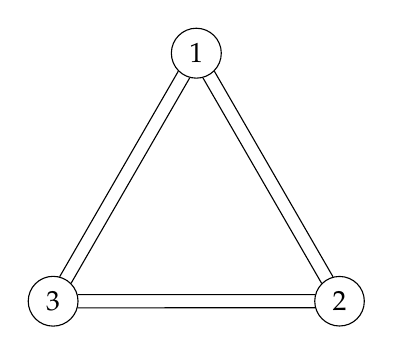
\begin{tikzpicture}[scale=.70]
\node[draw,circle] (A) at (90:3) {1};
\node[draw,circle] (B) at (210:3) {3};
\node[draw,circle] (C) at (330:3) {2};
\draw (A.225) -- node[rotate=60,above] {}  (B.75);
\draw(A.255) -- node[rotate=60,below] { } (B.45);
\draw (A.285) -- node[rotate=300,below] {} (C.135);
\draw  (A.315) -- node[rotate=300,above] {} (C.105);
\draw  (B.345) -- node[rotate=0,below] {} (C.195);
\draw  (B.15) -- node[rotate=0,above] {} (C.165);
\end{tikzpicture}
\qquad
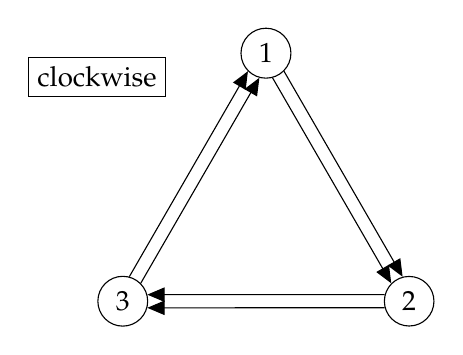
\begin{tikzpicture}[scale=.70]
\node[draw,circle] (A) at (90:3) {1};
\node[draw,circle] (B) at (210:3) {3};
\node[draw,circle] (C) at (330:3) {2};
\node[draw] (t) at (500:4) {clockwise};
\draw[triangle 45-] (A.225) -- node[rotate=60,above] {}  (B.75);
\draw[triangle 45-](A.255) -- node[rotate=60,below] { } (B.45);
\draw[-triangle 45] (A.285) -- node[rotate=300,below] {} (C.135);
\draw[-triangle 45]  (A.315) -- node[rotate=300,above] {} (C.105);
\draw[triangle 45-]  (B.345) -- node[rotate=0,below] {} (C.195);
\draw[triangle 45-]  (B.15) -- node[rotate=0,above] {} (C.165);
\end{tikzpicture}
\qquad
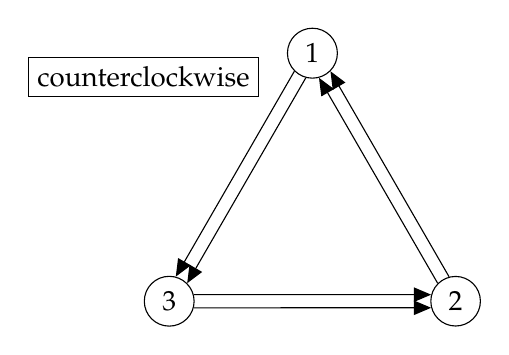
\begin{tikzpicture}[scale=.70]
\node[draw,circle] (A) at (90:3) {1};
\node[draw,circle] (B) at (210:3) {3};
\node[draw,circle] (C) at (330:3) {2};
\node[draw] (t) at (500:4) {counterclockwise};
\draw[-triangle 45] (A.225) -- node[rotate=60,above] {}  (B.75);
\draw[-triangle 45](A.255) -- node[rotate=60,below] { } (B.45);
\draw[triangle 45-] (A.285) -- node[rotate=300,below] {} (C.135);
\draw[triangle 45-]  (A.315) -- node[rotate=300,above] {} (C.105);
\draw[-triangle 45]  (B.345) -- node[rotate=0,below] {} (C.195);
\draw[-triangle 45]  (B.15) -- node[rotate=0,above] {} (C.165);
\end{tikzpicture}
$$
These houses have three rooms.  He can travel \emph{clockwise} (cw)
or \emph{counterclockwise} (ccw), as shown.

\newcommand{\cw}{\sw_{\mbox{\em cw}\ }}

\newcommand{\ccw}{\sw_{\mbox{\em ccw}\ }}

% \newcommand{\forces}{\,\mbox{$\mathrel\|\mathrel{\mkern-9mu}-\,$}}



We'd like to reason in this new setting.   So we make a logical language with operators 
$\cw$ and $\ccw$.   We call this language $\lang(\cw,\ccw)$.  

\begin{enumerate}
\item Fill in the chart below, telling what the semantics should be for this logic:

$$\begin{array}{l|l}
\begin{array}{lcl}
1\forces \cw\phi & \quadiff& \underline{\qquad\qquad}\\
2\forces \cw\phi & \quadiff& \underline{\qquad\qquad} \\
3\forces \cw\phi & \quadiff&\underline{\qquad\qquad} \\
\end{array}
\quad \quad & \quad \quad
\begin{array}{lcl}
1\forces \ccw\phi & \quadiff& \underline{\qquad\qquad} \\
2\forces \ccw\phi & \quadiff&\underline{\qquad\qquad} \\
3\forces \ccw\phi & \quadiff&\underline{\qquad\qquad} \\
\end{array}  \\
\end{array}
$$



\item
In the $\sw$-logic, we had sound logical principles such as
involution ($ \sw\sw\phi\iiff \phi$) and determinacy ($\nott\sw\phi\iiff\sw\nott\phi$).
What are the corresponding sound principles for  $\lang(\cw,\ccw)$?


\item   Suppose we want a proof system for validity, as we have done with our other logics.
How should the proof system work regarding subproofs?

\item Prove what you said in part (2) in the system which you constructed in part (3).
 {\bf New Point}
 Or, if your answer to part (3) was to make all of the sentences in part (2) to be axioms,
 you should prove something a little different.   For example,
 \[
\begin{array}{l}
 \proves (\ccw \phi) \iif (\cw\cw \phi) \\
  \proves (\cw\cw \phi) \iif (\ccw \phi)  \\
\proves (\cw\ccw)\phi \iif \phi\\
\end{array}
\]
 

%\item Sketch a proof of the completeness of your proof system.
%It should be closely based on the work we did for $\lang(\sw)$.


\end{enumerate}

\newcommand{\eat}{\poss_{\scriptstyle eat}\,}

\section{Eating}

Let's go back to $\lang(\sw)$.  Suppose that 
we wish to add a new action, $\eat$.
We want this action to correspond in a given room
to there bing food in that room, and then having  Ronnie eating all of it up.

So now we have a new syntax, giving us a language $\lang(\sw,\eat)$.   We get sentences like
\[\eat(\sw \mbox{water} \andd \eat\ \mbox{food}).\]

Now we turn to the semantics.   We need to say what it means to say that 
\[ i \forces\phi \mbox{ in $M$} \]
Where $M$ is a model (a two-room house), and $i$ is one of its two rooms, and $\phi$ is a sentence in our new language  $\lang(\sw,\eat)$.
For a model $M$, let $M_{-{\scriptsize food},i}$ be
the same as $M$, except that we change the valuation so that room $i$ contains no food.


\newcommand{\textfood}{\mbox{food}}

\newcommand{\textmaze}{\mbox{maze}}

\newcommand{\textwater}{\mbox{water}}

\newcommand{\texttreadmill}{\mbox{treadmill}}
For example, if $M$ is 
$$
 
\begin{tikzpicture}[<->,>=stealth',shorten >=1pt,auto,node distance=10cm,semithick]
\tikzstyle{every ellipse node}= [draw, text width = 2cm]
 \path  (-3,4.1) node[ellipse,text centered]  (v) {1:  $\textfood$, $\textmaze$};
  \path  (3,4.1) node[ellipse,text centered]  (w) {2:  $\textfood$, $\texttreadmill$};


\path[->] (v) edge node { }  (w);
\path[->] (1.4,3.92)  edge node {} (-1.4,3.92) ;

%\draw (x) -- (s) [swap] node[midway,below]   {a,b};
% \draw[<->]  (x) -- {a,b} (y);
%\path[->] (x) edge [loop left]  node {a,b} (x);
%\path[->] (s) edge [loop right] node {a,b} (s);
%\path[->] (z) edge [loop above] node {a} (z);
%\path[->] (v) edge [loop left] node {a} (v);
%\path[<-] (start) edge node  [swap] {b} (v);
%\path[<-](start) edge node [swap]  {c} (w);
%\path[<-](v) edge [bend right] node [near start,swap] {a} (x);
%\path[<-](x) edge [bend right] node [near start,swap] {b} (v);;
%\path[->](w) edge node [near start,swap] {a} (x);
%\path[<-](w) edge node [swap]  {c} (s);
%\path[<-](start) edge  [swap] node  {c} (s);
 \end{tikzpicture}
 $$
Then  $M_{-{\scriptsize food},1}$ is
$$
 
\begin{tikzpicture}[<->,>=stealth',shorten >=1pt,auto,node distance=10cm,semithick]
\tikzstyle{every ellipse node}= [draw, text width = 2cm]
 \path  (-3,4.1) node[ellipse,text centered]  (v) {1:    $\textmaze$};
  \path  (3,4.1) node[ellipse,text centered]  (w) {2:  $\textfood$, $\texttreadmill$};


\path[->] (v) edge node { }  (w);
\path[->] (1.4,3.92)  edge node {} (-1.4,3.92) ;

%\draw (x) -- (s) [swap] node[midway,below]   {a,b};
% \draw[<->]  (x) -- {a,b} (y);
%\path[->] (x) edge [loop left]  node {a,b} (x);
%\path[->] (s) edge [loop right] node {a,b} (s);
%\path[->] (z) edge [loop above] node {a} (z);
%\path[->] (v) edge [loop left] node {a} (v);
%\path[<-] (start) edge node  [swap] {b} (v);
%\path[<-](start) edge node [swap]  {c} (w);
%\path[<-](v) edge [bend right] node [near start,swap] {a} (x);
%\path[<-](x) edge [bend right] node [near start,swap] {b} (v);;
%\path[->](w) edge node [near start,swap] {a} (x);
%\path[<-](w) edge node [swap]  {c} (s);
%\path[<-](start) edge  [swap] node  {c} (s);
 \end{tikzpicture}
 $$
and 
 $(M_{-{\scriptsize food},1})_{-{\scriptsize food},2}$ is
$$
 
\begin{tikzpicture}[<->,>=stealth',shorten >=1pt,auto,node distance=10cm,semithick]
\tikzstyle{every ellipse node}= [draw, text width = 2cm]
 \path  (-3,4.1) node[ellipse,text centered]  (v) {1:    $\textmaze$};
  \path  (3,4.1) node[ellipse,text centered]  (w) {2:  $\texttreadmill$};


\path[->] (v) edge node { }  (w);
\path[->] (1.4,3.92)  edge node {} (-1.4,3.92) ;

%\draw (x) -- (s) [swap] node[midway,below]   {a,b};
% \draw[<->]  (x) -- {a,b} (y);
%\path[->] (x) edge [loop left]  node {a,b} (x);
%\path[->] (s) edge [loop right] node {a,b} (s);
%\path[->] (z) edge [loop above] node {a} (z);
%\path[->] (v) edge [loop left] node {a} (v);
%\path[<-] (start) edge node  [swap] {b} (v);
%\path[<-](start) edge node [swap]  {c} (w);
%\path[<-](v) edge [bend right] node [near start,swap] {a} (x);
%\path[<-](x) edge [bend right] node [near start,swap] {b} (v);;
%\path[->](w) edge node [near start,swap] {a} (x);
%\path[<-](w) edge node [swap]  {c} (s);
%\path[<-](start) edge  [swap] node  {c} (s);
 \end{tikzpicture}
 $$
 
Now we define:
\[
\begin{array}{lcl}
i\forces \eat\phi  \mbox{ in $M$} & \quadiff&  \mbox{food $\in \val_M(i)$,} \mbox{  and also $i \forces \phi $  in $M_{-{\scriptsize food},i}$}
\\
\end{array}  \\
\]
Note that if we have a model $M$ where there is no food in room $i$, then $i\forces \eat\phi$ is false in $M$.



With $M$ as above, tell whether the following are true or false, with reasons:
\begin{enumerate}
\item $1 \forces \eat \textfood$ in $M$.
\item $1 \forces \eat \sw\eat \true$ in $M$.
\end{enumerate}
And which of the following  are valid (true at all rooms of all models)?
\begin{enumerate}
\item[3.] $\eat\ \nott\textfood$
\item[4.] $\eat\ \textfood$
\item[5.] $(\eat\ \textwater) \iiff (\textfood\andd\textwater)$.
\end{enumerate}

\section{Eliminating $\eat$}

We say that two sentences, $\phi_1$ and $\phi_2$,
 in modal logic are \emph{semantically equivalent} if for every model $M$ and every world 
 $w$ in it,
$w\forces \phi_1$ if and only if $w \forces \phi_2$.

So for the logic $\lang(\sw,\eat)$, two sentences are semantically equivalent if 
for every rat house, each rom $i$ satisfies one of our sentences if and only if it satisfies the other.

\bigskip

Prove that for every sentence $\phi$ of $\lang(\sw,\eat)$ there is a sentence $\widehat{\phi}$ of $\lang(\sw)$
such that $\phi$ and $\widehat{\phi}$ are logically equivalent.

You should give a recursive definition of  $\widehat{\phi}$ as a function of $\phi$.
In other words, in defining  $\widehat{\phi}$, you can use  $\widehat{\psi}$ for various subsentences of $\phi$.

You don't have to prove your answer correct by induction (but that would be nice); you should just 
say what the main steps of the proof would be.

{\bf Clarification}
This problem will be really hard to do in full, unless you know some rather advanced topics.
What you should try to do is to write down \emph{recursion equations for the elimination of $\eat$}.
That is, you want to come up with facts like the following:
\[
\begin{array}{lcl}
\eat\ \textwater & \iiff & \textfood \andd\textwater \\
\eat \eat \phi  & \iiff & \false \\
\end{array}
\]
The point is that these two sentences are valid (true in every room of every house).
And so part of the definition of $\widehat{\phi}$ will be 
\[
\begin{array}{lcl}
(\eat\ \textwater)^{\hat{}}& = & \textfood \andd\textwater \\
(\eat \eat \phi )^{\hat{}} & = & \false \\
\end{array}
\]
(I have written  $\widehat{\phi}$ as $\phi^{\hat{}}$ for typographic reasons.)

And you also will have equations like
\[
\begin{array}{lcl}
(\phi\andd\psi)^{\hat{}}& = & \phi^{\hat{}} \andd \psi^{\hat{}}\\
%(\eat \eat \phi )^{\hat{}} & = & \false \\
\end{array}
\]

It would be really nice if you could have enough recursion equations to ``cover all the cases''.
That is, you want to have enough equations that \emph{every sentence in the new language $\lang(\sw,\eat)$ is covered
by one of your equations}.

\rem{
{\bf Note} In this homework, and in all work in this class: unless otherwise stated,
you may use the soundness or completeness of a proof system.
But whenever you do, you need to say which one you are using.


\section{de Morgan's Laws}
 

\begin{enumerate}
\item Give a derivation that shows $\proves\nott(\phi\andd\psi)\iif (\nott \phi)\orr (\nott\psi)$.
\item Give a derivation that shows $\proves(\nott \phi)\orr (\nott\psi) \iif \nott(\phi\andd\psi)$.
\end{enumerate}
In one of the two parts, you will need to use the Law of the Excluded Middle.

\section{Satisfiability in propositional logic}
Recall that  a propositional logic sentence
$\phi$ is \emph{satisfiable} if there is some valuation $v$ such that $\semantics{$\phi$}_v =\true$.

For each of the following sentences, tell whether true
or false.  For the true ones, give a short proof.
For the false ones, give a counterexample.
\begin{enumerate}
\index{satisfiable!in propositional logic}
\item Every sentence $\phi$ or its negation $\nott\phi$ is satisfiable.
\item Both $\phi$ and $\nott\phi$ are satisfiable. \label{partb}
\item If $\phi\andd\psi$ is satisfiable, then both $\phi$ and $\psi$ are satisfiable. 
\item If  both $\phi$ and $\psi$ are satisfiable,
then $\phi\andd\psi$ is satisfiable.
\item If $\phi\orr\psi$ is satisfiable, then either $\phi$ or $\psi$
(or both) are satisfiable. 
\item If  either $\phi$ or $\psi$ is satisfiable,
then $\phi\orr\psi$ is satisfiable.
\item  If $\phi$ and $\phi\iif\psi$ are satisfiable, then $\psi$ is satisfiable.
\item Every sentence $\phi$ or its negation $\nott\phi$ is a tautology.
\item  If $\phi\andd\psi$ is a tautology, then both $\phi$ and $\psi$ are tautologies. 
\item If $\phi\orr\psi$ is a tautology, then either $\phi$ or $\psi$
(or both) are tautologies. 
\item If $\phi$ and $\phi\iif\psi$ are tautologies, then $\psi$ is a tautology.
\end{enumerate}
[As a hint, I'll solve the first two parts.
Part (1) is true for the following reason: 
Fix the sentence $\phi$.   Let $v$ be any valuation.
Either $\semantics{$\phi$}  = \true$ or $\semantics{$\phi$} = \false$.
In the first case, $v$ shows that $\phi$ is satisfiable.
In the second case, 
$$\semantics{$\nott\phi$}  = \nott \semantics{$\phi$}  = \nott \false  = \true,$$
and therefore $v$ shows that $\nott\phi$ is satisfiable.
On the other hand, part (\ref{partb}) is false.
We may take $\phi$ to be $p\andd\nott p$.  This sentence is not satisfiable.]

 


\section{Avoiding confusion}

It is easy to confuse 
the following two assertions:
\begin{enumerate}
\item[(i)]   $\not\proves \phi\iif \psi$ 
\item[(ii)]  $\proves \phi\iif \nott\psi$.
\end{enumerate}
(i) says that there is \emph{no} derivation in our system that has no premises and ends with $\phi\iif \psi$.
(ii) says that there  \emph{is} a  derivation in our system that has no premises and ends with $ \phi\iif \nott\psi$.

\begin{enumerate}
\item Give an example of two sentences $\phi$ and $\psi$ in propositional logic 
with the property that $\not\proves \phi\iif \psi$ but    $ \not\proves \phi\iif \nott\psi$.
This shows that (i) does not in general imply (ii).
\item Give an example of two sentences $\phi$ and $\psi$ in propositional logic 
with the property that $\proves \phi\iif \psi$ and also   $ \proves \phi\iif \nott\psi$.
This shows that (ii) does not in general imply (i).
\end{enumerate}

 
\section{A step in the lemma on state descriptions}
Recall from class the main lemma on state descriptions.
It says:   For all sentences $\phi$, 
and all state descriptions $\alpha$, 
if $\occ(\phi)\subseteq \occ(\alpha)$, then 
  either $\proves \alpha\iif \phi$, or else $\proves \alpha\iif \nott\phi$.

The proof was by induction on $\phi$.  In the lecture slides, you can find the induction steps for $\andd$ and for $\nott$.
Your task: prove the induction step for $\iif$.
Be sure to use the relation between the sets $\occ(\phi\iif\psi)$, $\occ(\phi)$, and $occ(\psi)$.


 \section{Consistent and satisfiable}
 
 A sentence $\phi$ in propositional logic  is \emph{consistent} if $\not\proves\nott \phi$.
That is, $\nott\phi$ is \emph{not} provable.  

\begin{enumerate}
\item 
Prove that if $\phi$ is consistent, then $\phi$ is satisfiable.
\item
Prove that if $\phi$ is satisfiable, then $\phi$ is consistent.
\end{enumerate}
You will need to use either the soundness or completeness of our logic, or both.
    Please be sure to write down exactly where
you used these results.
}


\end{document}
